\subsection{Process View}

\copied{Process view : The process view deals with the dynamic aspects of the system, explains the system processes and how they communicate, and focuses on the runtime behavior of the system. The process view addresses concurrency, distribution, integrators, performance, and scalability, etc. UML Diagrams to represent process view include the Activity diagram.}
{from wikipedia}
This view mainly discuss about runtime, concurrency, communication, and synchronization of the process running in the system. \\

The program flow and business logic of the system are captured in this section with the aid of several activity diagrams.

\subsubsection*{Flood monitoring}

The activity diagram in figure~\ref{fig:activity-monitoring} shows the flow of the flood monitoring process.


\begin{figure}[h]
\centering
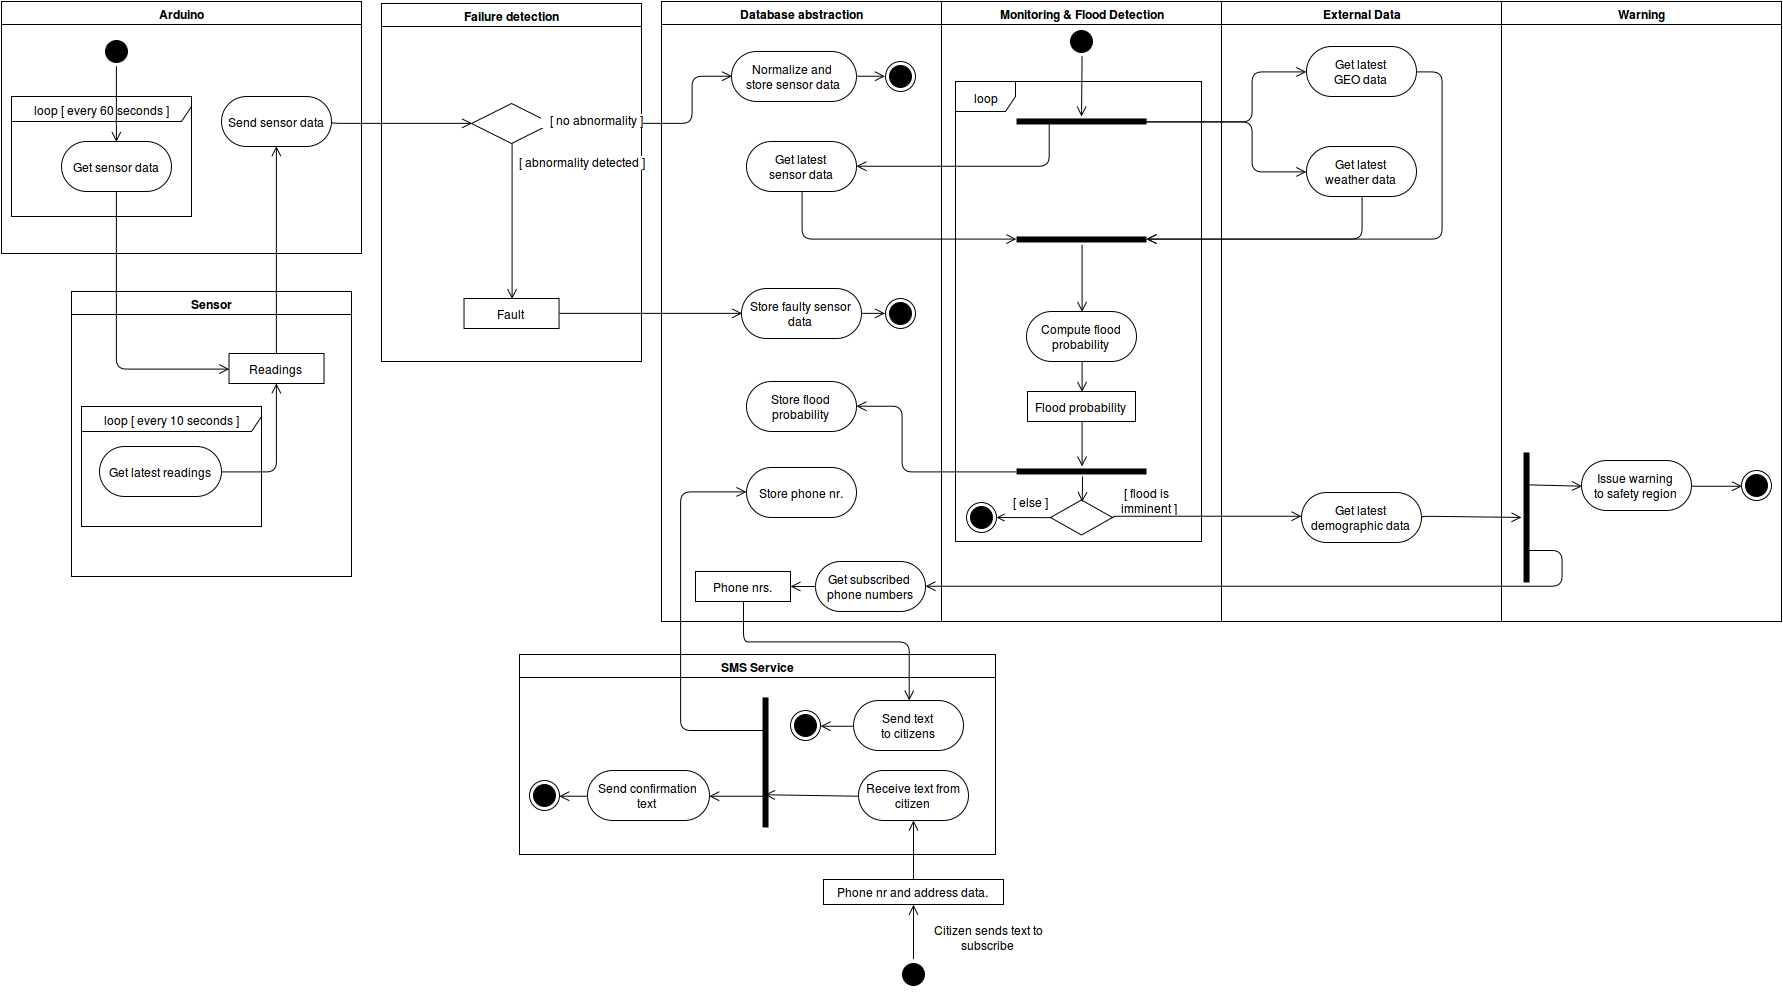
\includegraphics[keepaspectratio=true,width=1.0\textwidth]{{\viewimages/activity_monitoring}.png}
\caption{An activity diagram of the flood monitoring process}
\label{fig:activity-monitoring}
\end{figure}